\documentclass{article} % \documentclass{} is the first command in any LaTeX code.  It is used to define what kind of document you are creating such as an article or a book, and begins the document preamble

\usepackage{amsmath, listings, tikz, graphicx, float, bbm, hyperref, amssymb, setspace, indentfirst, dcolumn, booktabs, adjustbox}  % \usepackage is a command that allows you to add functionality to your LaTeX code
\usepackage[authoryear, round]{natbib}
\usepackage[margin=1in]{geometry}
\setcitestyle{aysep={,},yysep={,},citesep={;},maxcitenames=2}
%\usetikzlibrary{trees}

\title{Charter School Heterogeneity: CF Output Tables} % Sets article title
\author{Nicholas Lacoste} % Sets authors name
\date{\today} % Sets date for date compiled

% The preamble ends with the command \begin{document}
\begin{document} % All begin commands must be paired with an end command somewhere
    \maketitle % creates title using infromation in preamble (title, author, date)

\section{Graduation Rate Results}

Table 1:\\
% latex table generated in R 4.4.0 by xtable 1.8-4 package
% Mon Sep  9 19:41:55 2024
\begin{tabular}{rlrrr}
  \hline
 & Covariate & Significantly Positive & Significantly Negative & Difference (Positive - Negative) \\ 
  \hline
1 & Log of Enrollment & 7.56 & 7.35 & 0.21 \\ 
  2 & Percent White & 0.90 & 0.67 & 0.23 \\ 
  3 & Percent Black & 0.03 & 0.06 & -0.03 \\ 
  4 & Percent Hispanic & 0.04 & 0.21 & -0.17 \\ 
  5 & Percent Free/Reduced Lunch & 0.24 & 0.39 & -0.15 \\ 
  6 & Percent Special Ed & 0.13 & 0.12 & 0.01 \\ 
  7 & Urban & 0.05 & 0.03 & 0.01 \\ 
  8 & Suburb & 0.21 & 0.20 & 0.01 \\ 
  9 & Town & 0.22 & 0.20 & 0.02 \\ 
  10 & Rural & 0.52 & 0.56 & -0.04 \\ 
  11 & Per Pupil Revenue & 9112.63 & 8733.56 & 379.07 \\ 
  12 & Per Pupil Expenditure & 9155.10 & 8748.36 & 406.74 \\ 
  13 & Student-Teacher Ratio & 15.66 & 15.38 & 0.29 \\ 
  14 & Teacher Salary & 71827.03 & 69836.17 & 1990.86 \\ 
  15 & Number of Magnet Schools & 0.18 & 0.00 & 0.18 \\ 
  16 & Charter Effectiveness & 0.74 & 0.74 & 0.01 \\ 
  17 & Number of Observations & 5730.00 & 2727.00 & 8457.00 \\ 
   \hline
\end{tabular}



Table 2:\\
% latex table generated in R 4.4.0 by xtable 1.8-4 package
% Tue Sep 10 11:10:30 2024
\begin{tabular}{rlrrrr}
  \hline
 & Group & GATE & SE & p.value & X..N \\ 
  \hline
1 & Urban & 0.49 & 0.31 & 0.12 & 0.06 \\ 
  2 & Suburban & -0.18 & 0.18 & 0.32 & 0.23 \\ 
  3 & Rural & 0.55 & 0.60 & 0.36 & 0.52 \\ 
  4 & Percent Free Lunch $>$ 20\% & 0.37 & 0.20 & 0.07 & 0.60 \\ 
   \hline
\end{tabular}


Table 3:\\
% latex table generated in R 4.4.0 by xtable 1.8-4 package
% Tue Sep 10 13:21:31 2024
\begin{tabular}{lrrrr}
  \hline
Variable & Estimate & Std..Error & t.value & Pr...t.. \\ 
  \hline
(Intercept) & -6.73 & 1.49 & -4.51 & 0.00 \\ 
  logenroll & 0.52 & 0.12 & 4.15 & 0.00 \\ 
  perhsp & 0.19 & 0.49 & 0.38 & 0.70 \\ 
  perfrl & 2.53 & 1.16 & 2.18 & 0.03 \\ 
  perwht & 1.53 & 1.04 & 1.46 & 0.14 \\ 
  str & 0.01 & 0.04 & 0.22 & 0.83 \\ 
   \hline
\end{tabular}


Figure 1:\\
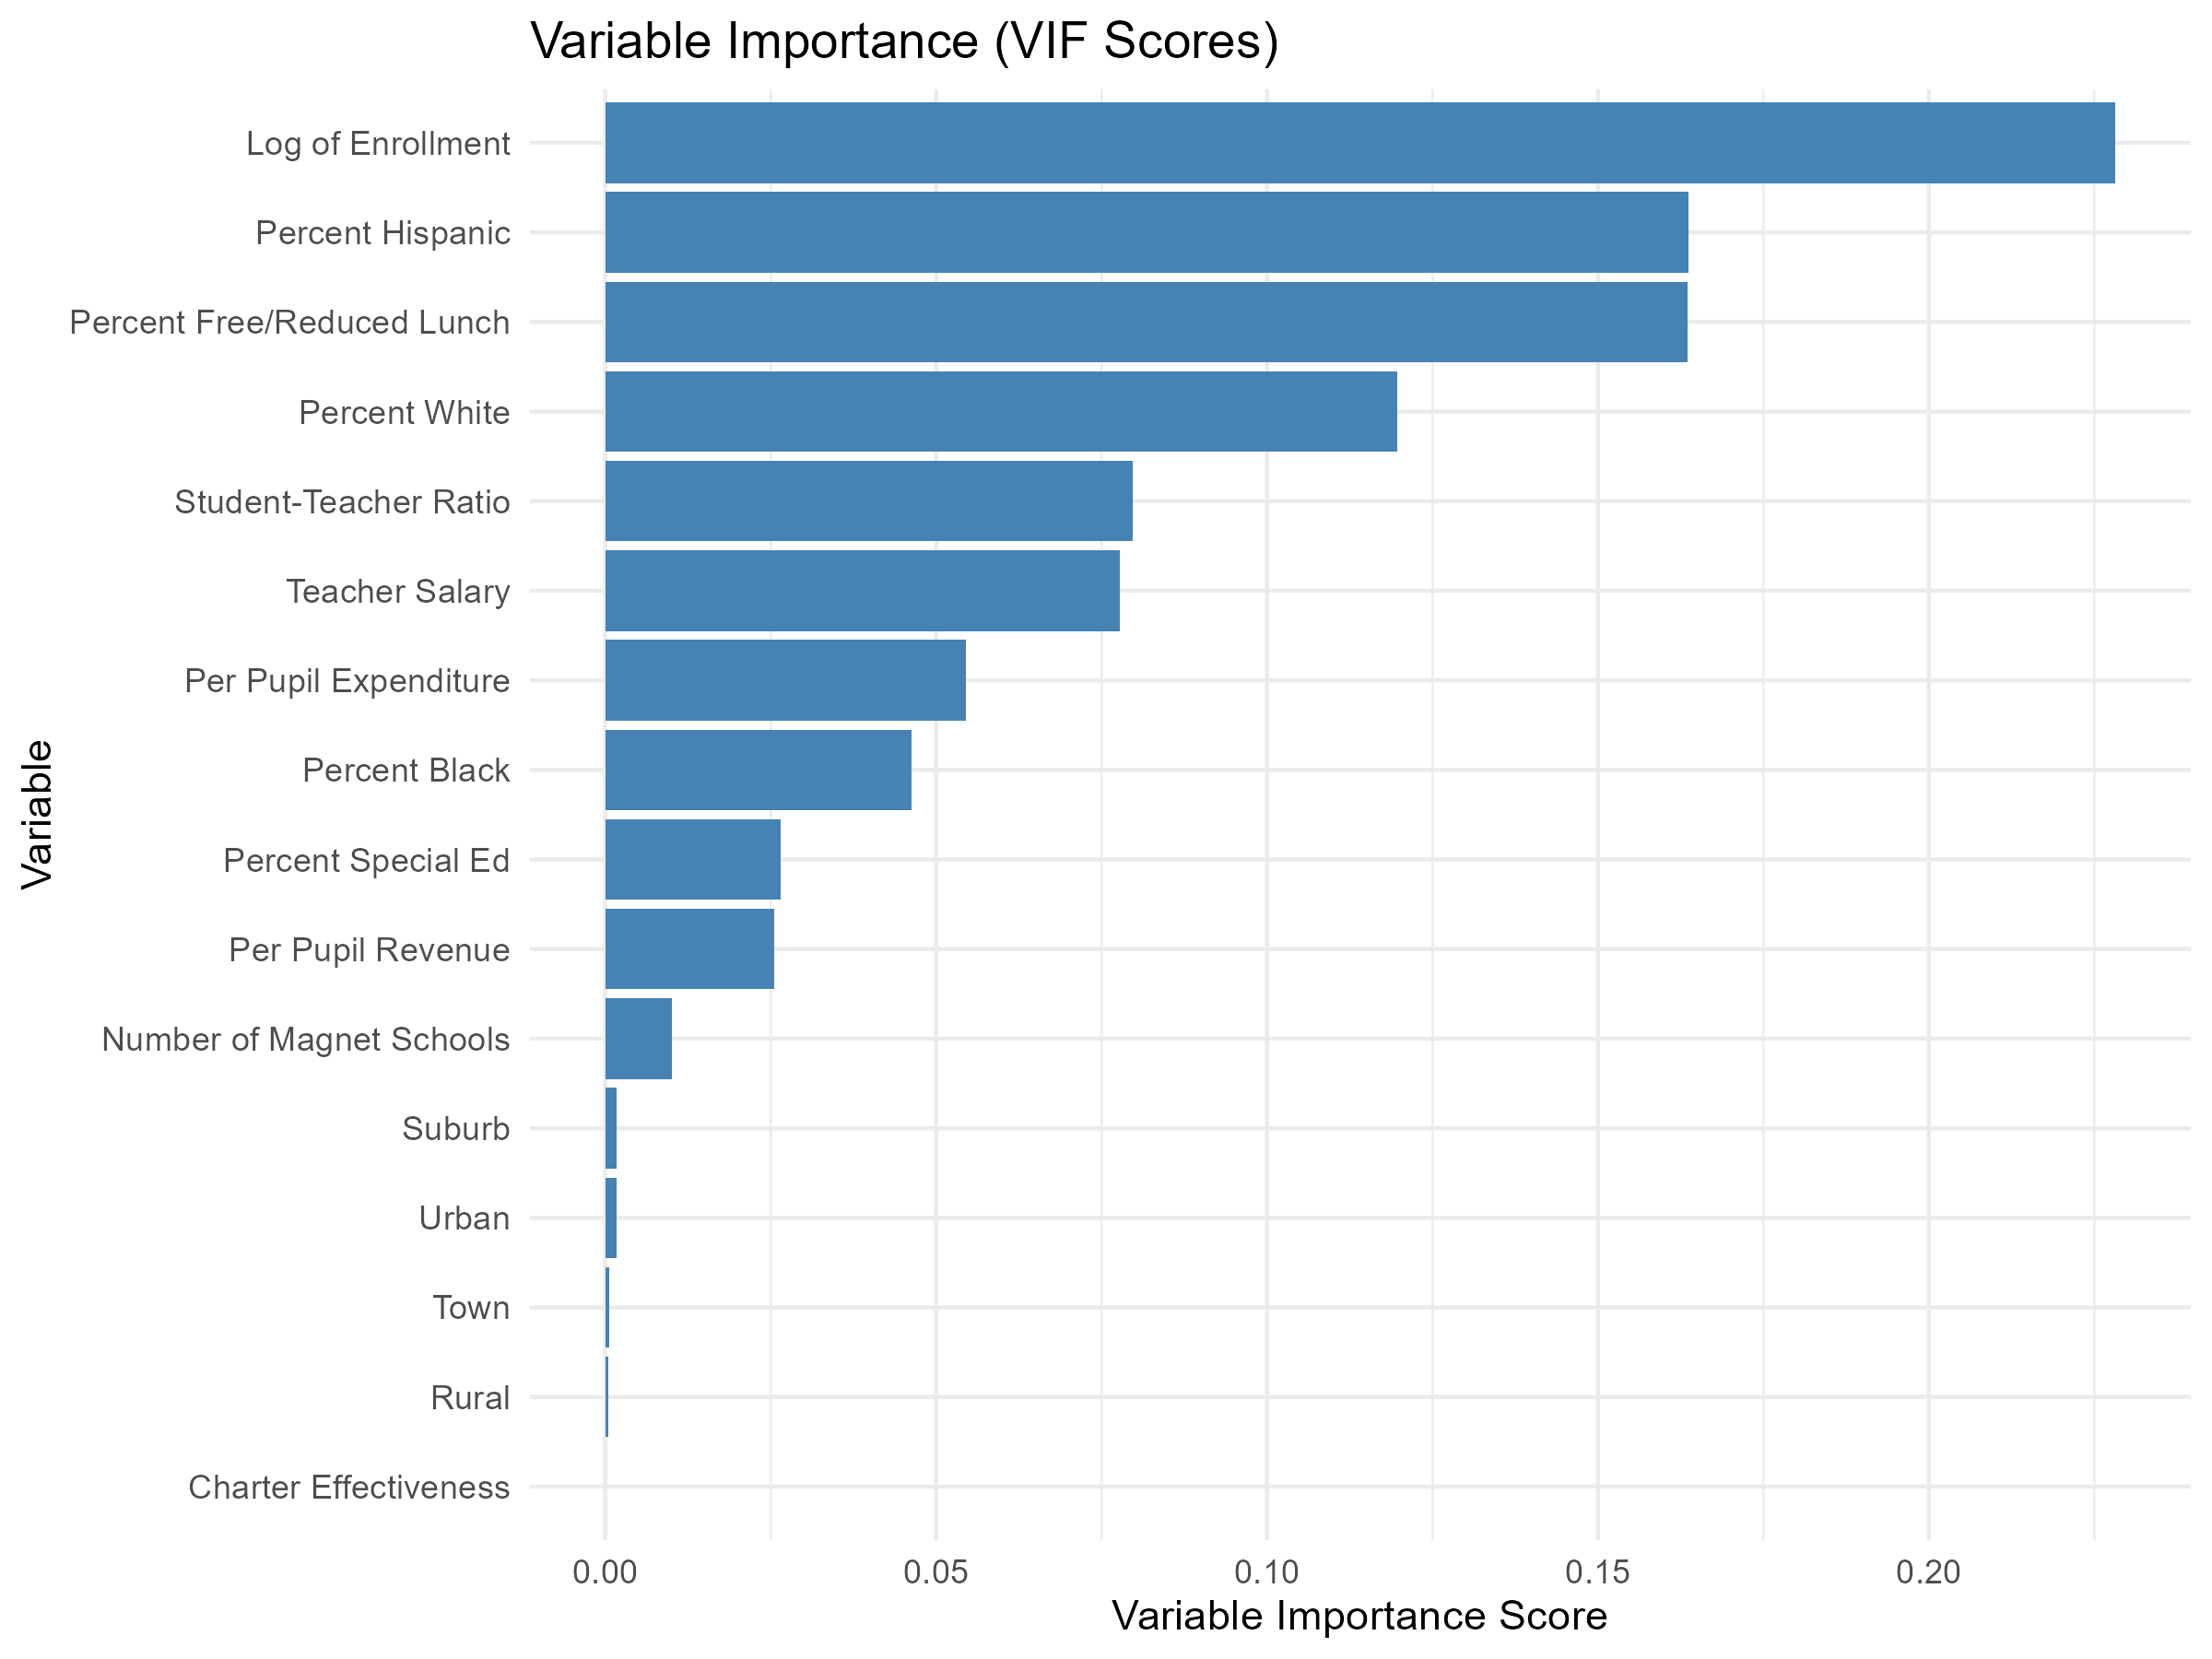
\includegraphics[width=\textwidth]{c:/Users/nickm/OneDrive/Acer (new laptop)/Documents/PhD/Tulane University/Projects/Charter School Heterogeneity/Charter_School_Heterogeneity_Project/analysis/output/vif_scores.png}
	
Figure 2:\\
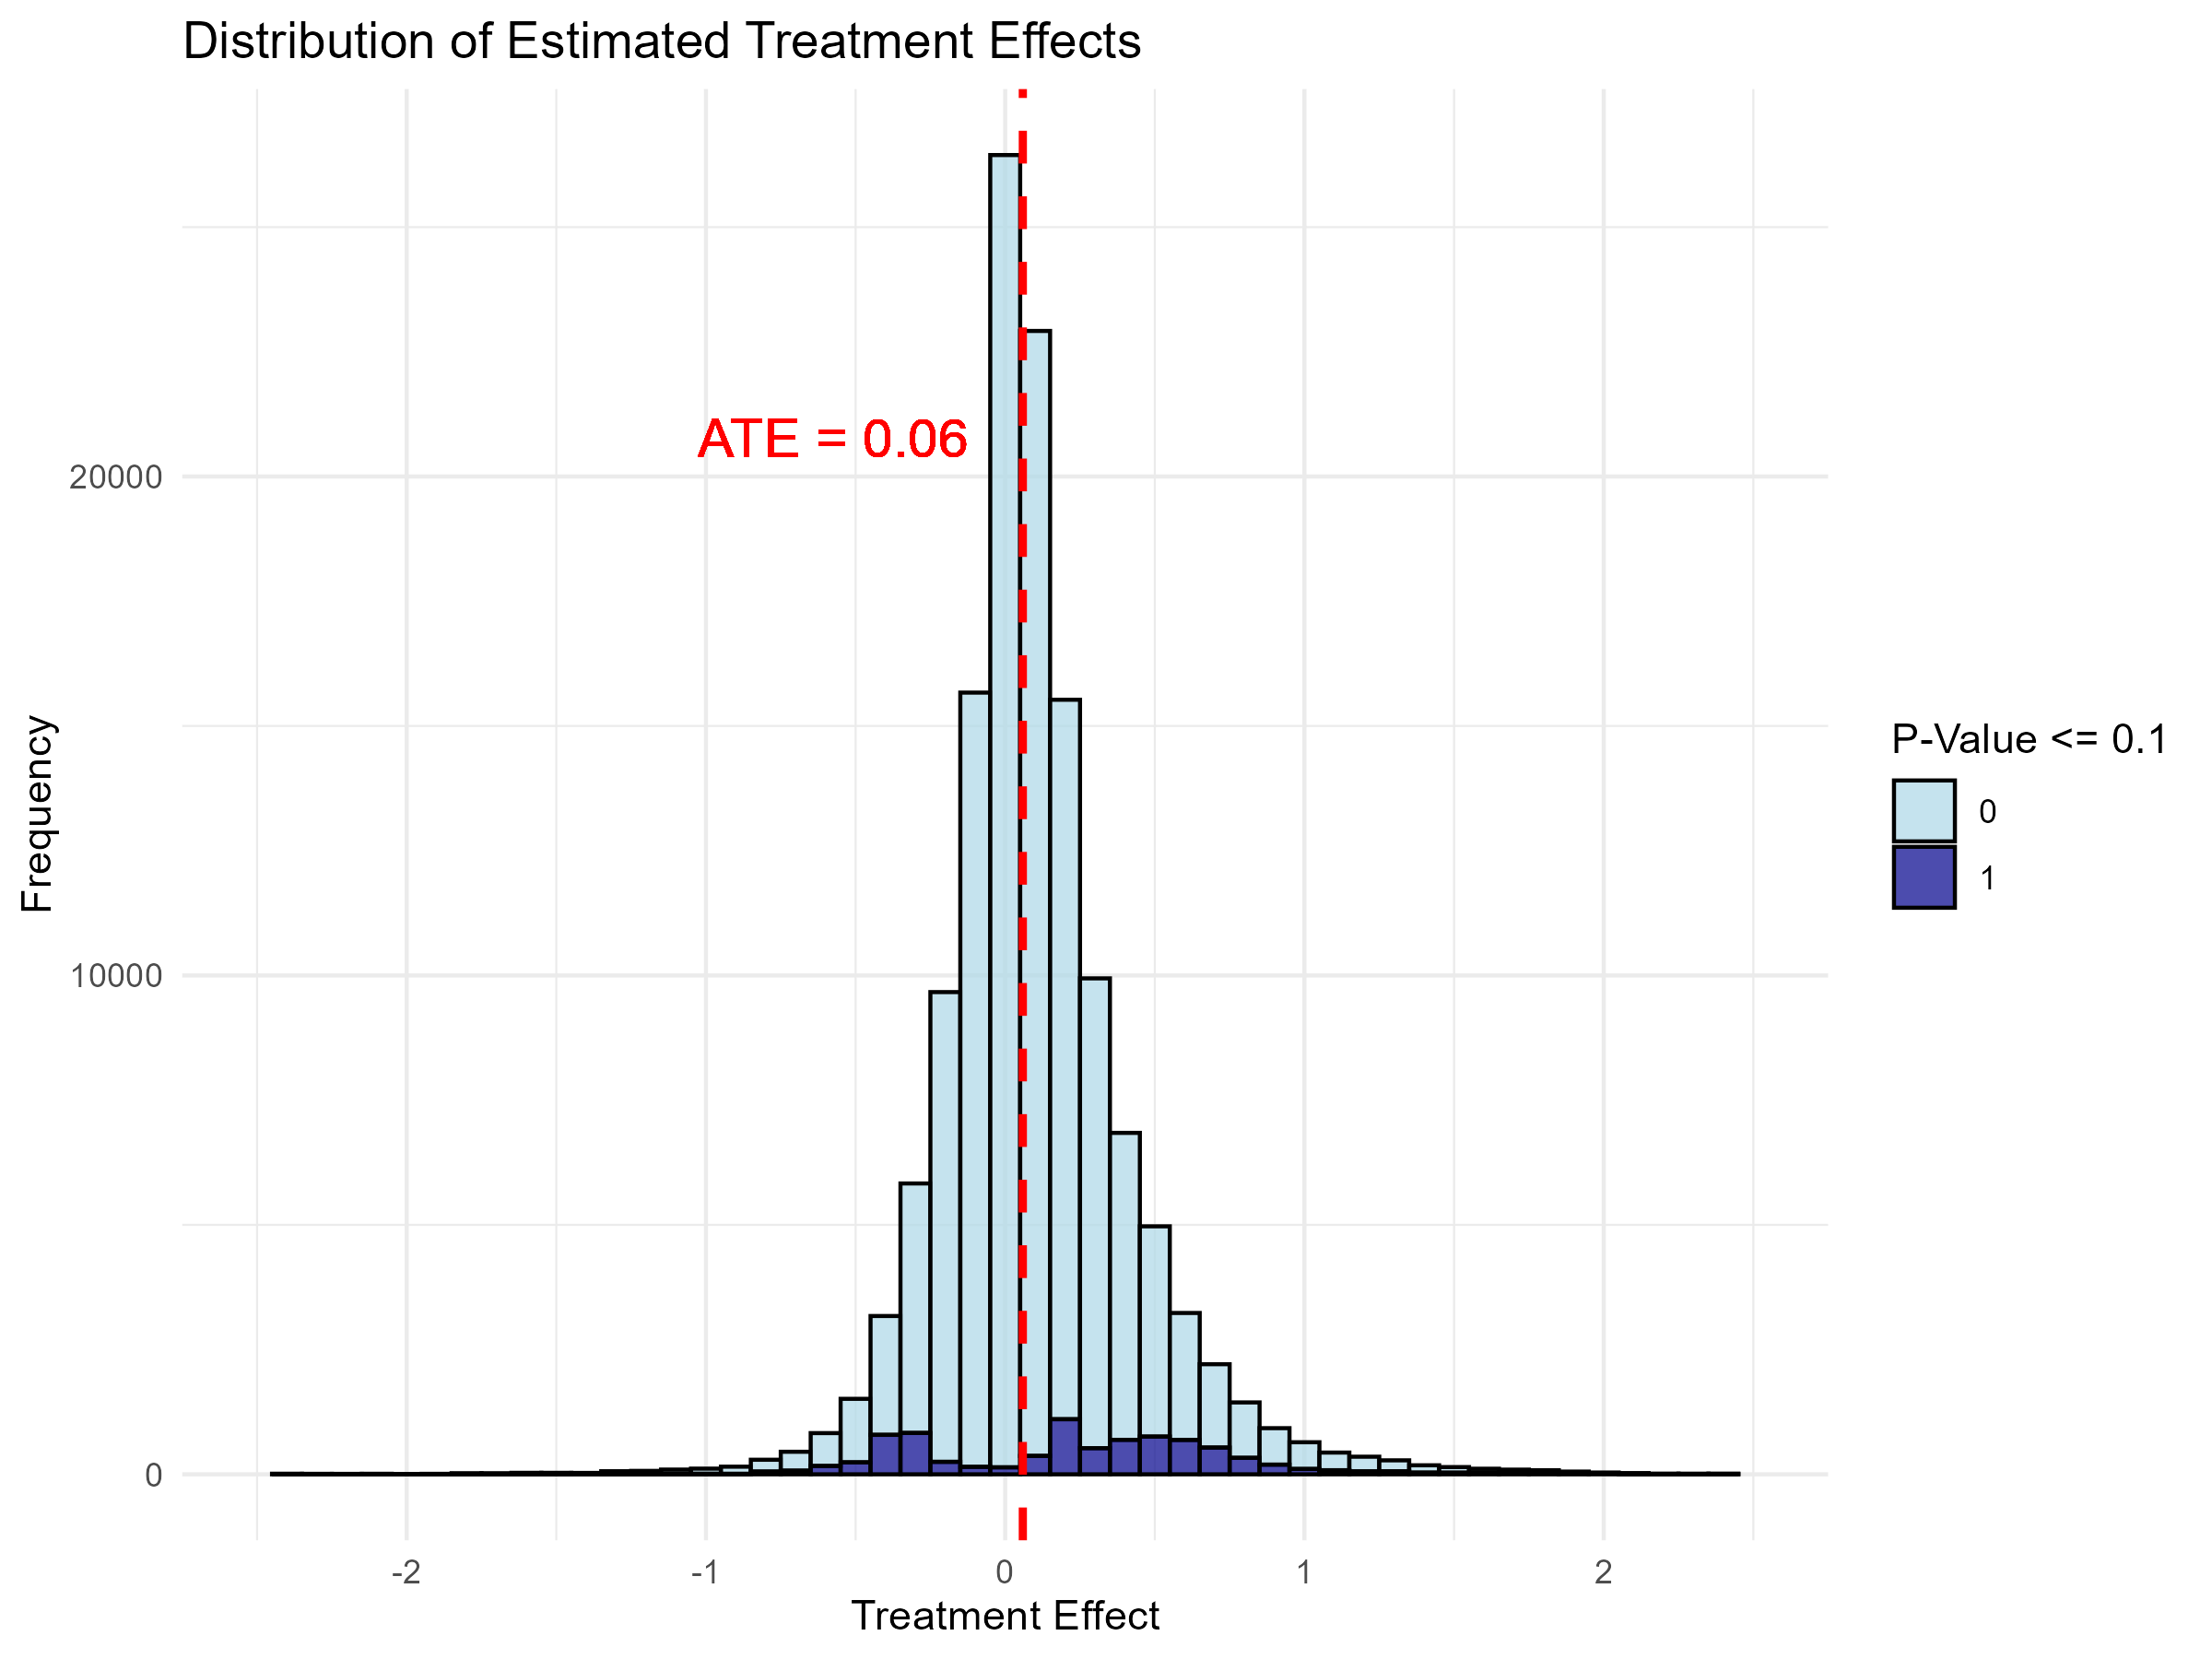
\includegraphics[width=\textwidth]{c:/Users/nickm/OneDrive/Acer (new laptop)/Documents/PhD/Tulane University/Projects/Charter School Heterogeneity/Charter_School_Heterogeneity_Project/analysis/output/afgr_cate_dist.png}

\section{Test Scores Results}
	
	

	
	

	
	

	
	
	 
	

	
	
	


	




	 

 













\end{document} % This is the end of the document